\documentclass{article}
\usepackage{tikz}
\usepackage{xcolor}

\definecolor{myblue}{RGB}{40,110,160}
\definecolor{bggray}{RGB}{245,245,245}
\definecolor{gridgray}{RGB}{180,180,180}

\begin{document}

\begin{center}
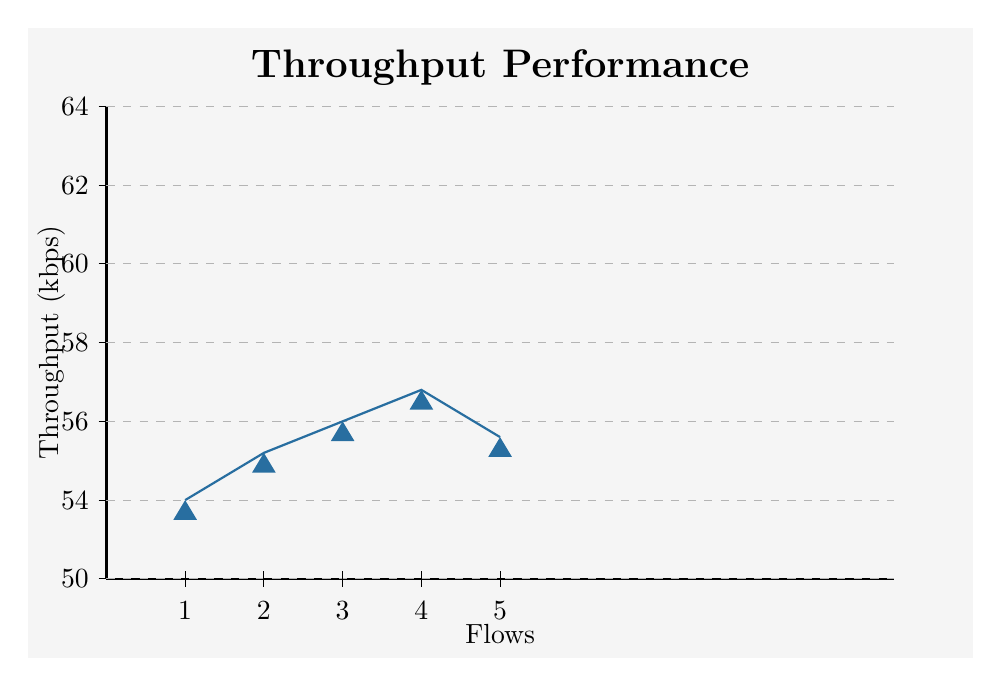
\begin{tikzpicture}

% Background
\fill[bggray] (0,0) rectangle (12,8);

% Axes
\draw[thick] (1,1) -- (1,7);
\draw[thick] (1,1) -- (11,1);

% Title
\node[font=\Large\bfseries] at (6,7.5) {Throughput Performance};

% Axis labels
\node[rotate=90] at (0.3,4) {Throughput (kbps)};
\node at (6,0.3) {Flows};

% Y-axis ticks
\foreach \y/\val in {
1/50,
2/54,
3/56,
4/58,
5/60,
6/62,
7/64
}{
\draw (0.9,\y) -- (1.1,\y);
\node[left] at (0.9,\y) {\val};
\draw[dashed, gridgray] (1,\y) -- (11,\y);
}

% X-axis ticks
\foreach \x/\val in {
1/1,2/2,3/3,4/4,5/5
}{
\draw (\x+1,0.9) -- (\x+1,1.1);
\node at (\x+1,0.6) {\val};
}

% Scale factor (maps values to Y axis)
\def\scale{0.2}

% Plot line
\draw[thick, myblue]
(2,{1+(55-50)*\scale}) --
(3,{1+(58-50)*\scale}) --
(4,{1+(60-50)*\scale}) --
(5,{1+(62-50)*\scale}) --
(6,{1+(59-50)*\scale});

% Triangle markers
\foreach \x/\y in {
2/55,
3/58,
4/60,
5/62,
6/59
}{
\fill[myblue] (\x,{1+(\y-50)*\scale}) -- ++(-0.15,-0.25) -- ++(0.3,0) -- cycle;
}

\end{tikzpicture}
\end{center}

\end{document}